\subsection{Vista}

La vista contiene los componentes para representar la interfaz del usuario (IU) del programa y las herramientas con las cuales el usuario puede interactuar con los datos de la aplicación. Adicionalmente, la vista se encarga de recibir e interpretar adecuadamente los datos obtenidos del modelo. Cabe mencionar, que al igual que el resto de componentes del MVC, la clase View implementa la interfaz \say{Notify}, la cual permite la comunicación con el resto de elementos.\bigskip

\texttt{loadContent} es el encargado de cargar el contenido inicial en la ventana. Para esta práctica, carga los siguientes elementos semánticos:\bigskip

\texttt{menu}, función que crea y configura el menú de utilidades de la ventana principal. En esta, se incluyen las siguientes opciones: Abrir ventanas de estadísticas y salir del programa.\bigskip

\texttt{body}, función que crea, configura y actualiza la gráfica de la ventana principal. Se trata de un mapa en el que se pueden seleccionar los puntos o poblaciones, estos puntos están conectados por una serie de caminos. Para ello, se han usado las clases JFreeChart, y una clase que hemos creado para añadir elementos sobre el mapa, MapPlot. \bigskip

\texttt{sidebar}, función que crea y configura la barra de opciones de la derecha de la interfaz principal. Esta permite al usuario interactuar y configurar el entorno de ejecución de los algoritmos y seleccionar los mapas configurados. Además, se ha añadido una pequeña ventana de logs para saber que está ocurriendo en todo momento.\bigskip

\texttt{footer}, función que crea y configura los botones para manipular los puntos seleccionados sobre el mapa. El botón Deshacer, elimina el último punto añadido. El botón Rehacer, añade el último punto borrado. El botón Limpiar elimina todos los datos añadidos sobre el mapa. Por último, el botón Confirmar ejecuta el algoritmo y encuentra un camino óptimo entre los puntos seleccionados. \bigskip

Adicionalmente, a la vista principal, esta permite desplegar dos ventanas más. Una ventana muestra a tiempo real, el uso y consumo de la memoria de la Java virtual machine (JVM) y la otra ventana muestra las estadísticas de la ejecución de los algoritmos además de su comparación. A continuación, se muestran dos imágenes (\ref{fig:Ejemplo stats JVM} y \ref{fig:Ejemplo stats Algt}) de como se verían las ventanas al iniciarlas junto a una breve explicación de la misma.

Finalmente, al ser un módulo de nuestro MVC, implementa la interfaz \texttt{Notify} y su método \texttt{notifyRequest} que le permite recibir notificaciones de los otros módulos del MVC.

\subsubsection{Estadísticas JVM}\label{Stats JVM}

Este apartado de la vista principal, es el encargado de enseñar a tiempo real las estadísticas de la máquina virutal de java. Concretamente, se actualiza cada 0.5s a apartir de los datos obtenidos de la clase de java \say{Runtime} y muestra la memoria libre, la memoria total y el uso de esta en una gráfica de lineas, donde el eje x es instante en el tiempo que se han obtenido los datos y el eje y su valor. Todos los datos de la memoría obtenidos están en MB.

\begin{figure}[!h]
    \centering
    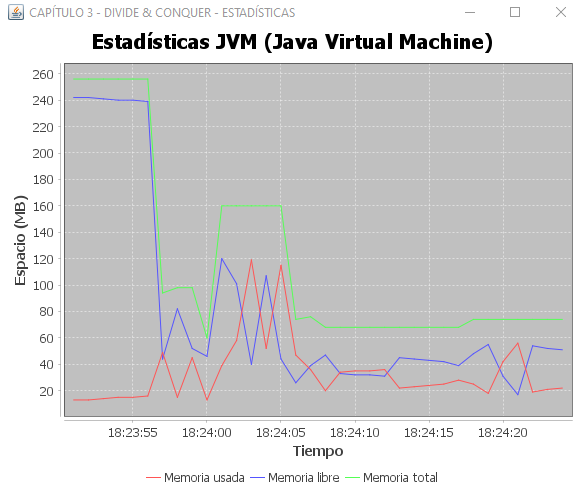
\includegraphics[width=\linewidth]{MVC/View/img/stats-jvm.png}
    \caption{Interfaz estadísticas JVM}
    \label{fig:Ejemplo stats JVM}
\end{figure}

\subsubsection{Estadísticas Algoritmos}\label{Stats Algt}

Este apartado de la vista principal, es el encargado de enseñar las estadísticas de la ejecución de los algoritmos, $Dijkstra$.... Estas estadísticas incluyen dos gráficas, las estadísticas por iteración y las estadísticas globales, ambas de la ejecución del algoritmo con la distancia seleccionada. En la gráfica por iteración se encuentran los datos obtenidos de cada ejecución por separado del algoritmo, concretamente, el número de iteraciones que ha realido esa ejecución, cuantos nodos se ha visitado en cada iteración y la memoria empleada. Y en la otra gráfica, se muestra el tiempo que ha tardado en encontrar la solución, los nodos visitados de media, la memoria media empleada, el número de iteraciones medio por ejecución del algoritmo y la cantidad de nodos que tiene el grafo. 

\begin{figure}[!h]
    \centering
    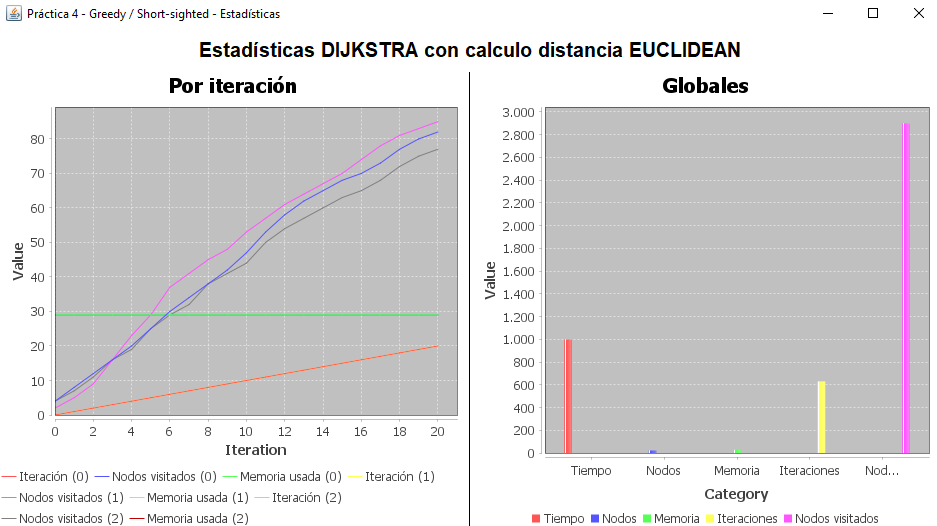
\includegraphics[width=\linewidth]{MVC/View/img/stats-algt.png}
    \caption{Interfaz estadísticas algortimos}
    \label{fig:Ejemplo stats Algt}
\end{figure}

Como se ha podido ver anteriormente en la imagen (\ref{fig:Ejemplo stats Algt}), los datos de las estadísticas están representados con un diagrama de barras y un diagrama de lineas, donde el eje x es la categoría a la que pertenecen y el eje y el valor correspondiente, en la caso de la segunda gráfica. En el caso de la primera gráfica, el eje X es la iteración y el eje y el valor.
